\documentclass[9pt]{extarticle}

\usepackage{blindtext}

% Handle enumeration list
\usepackage{enumitem}

% Citations as footnotes
% \usepackage[style=verbose,backend=bibtex]{biblatex}
% \bibliography{refs.bib}

\usepackage{amsmath}
\usepackage{amssymb}
\usepackage{graphicx}
\usepackage{microtype}

% Directory for images
\graphicspath{{images/}}

% To wrap text around figures
\usepackage{wrapfig}

% Define new type of columns
\usepackage{array}
\usepackage{tabulary}
\newcolumntype{K}[1]{>{\centering\arraybackslash}m{#1}}

% Stretch the dimension of the rows in tables
\renewcommand{\arraystretch}{1.6}

% Add colors to table
\usepackage{colortbl}

% Set Helvetica as main font
\usepackage{helvet}
\renewcommand\familydefault{\sfdefault}
\usepackage[T1]{fontenc}

% Set Helvetica as main font for equations
\usepackage[helvet]{sfmath}

% Set Helvetica as main font for equations (alternative)
% \usepackage{eulervm}

% Change geometry of the page
\usepackage[left=2cm,top=2cm,right=1.5cm,bottom=1.5cm]{geometry}

% Change spacing
\usepackage{setspace}
\onehalfspacing

\usepackage[svgnames]{xcolor}
\usepackage[pdftex]{hyperref}
\hypersetup{colorlinks=true,linkcolor=blue,citecolor=ForestGreen,urlcolor=DarkOrchid}

% Where images are located
\graphicspath{{images/}}

% Redefine names
\newcommand{\sectionname}{Section}
\renewcommand{\appendixname}{Appendix}
\newcommand{\equationname}{Equation}
\newcommand{\referencename}{Ref.}
\renewcommand{\figurename}{Figure}
\renewcommand{\tablename}{Table}

% Adjust section titles
\usepackage{titlesec}
\titleformat{\section}{\bfseries\normalsize}{\thesection.}{0.5em}{}

% Change position of the page number
\usepackage{fancyhdr}
\pagestyle{fancy}
\renewcommand{\headrulewidth}{0pt}
\fancyhf{}
\fancyhead[R]{\thepage}

% Add notes to the text
\usepackage{changes}
\newcommand{\note}[1][]{\added[remark={#1}]}

% Some useful definition
\newcommand{\DW}{\mbox{D-Wave 2X\textsuperscript{TM}}~}

\begin{document}

\begin{center}\Large
\textbf{\note[Feel free to shuffle the order of the authors]{Exploration} of the Potential of Quantum Annealing for Hard Scheduling
Problems in Air Traffic Management: Report, April-July 2016 (3.5 months)}
\end{center}

\def\changemargin#1#2{\list{}{\rightmargin#2\leftmargin#1}\item[]}
\let\endchangemargin=\endlist 

\section*{Introduction}\label{sec:intro}

\hspace{-0.23cm}\begin{tabular}{p{9cm}p{0.1cm}p{8cm}}
\vspace{-5.3cm}
Given encouraging of early results in the planning domain \cite{rieffel:15,venturelli:15}
and the expertise of our team in such sector, 
aim of the project is to explore the potential use of the Quantum Annealing (QA), and in particular of the state-of-art \DW quantum annealer hosted at NASA Ames, 
as a metaheuristic for solving computational challenging problems in the context of
Air Traffic Management (ATM) \cite{rodionova:16, rodionova:thesis15}. More precisely, the project has been focused on the problem to reduce the number
of potential enroute conflicts of wind-optimal trajectories. 
In this project, we limit our attention to the North Atlantic oceanic airspace (NAT) for which we have wind-optimal trajectories
for two consecutive days (July 28\textsuperscript{th}-29\textsuperscript{th} 2012). The project has been conducted by experts of the QuAIL team
(Tobias Stollenwerk, Bryan O'Gorman, Salvatore Mandr\`a, Davide Venturelli and Eleanor G. Rieffel), in close collaboration with
ATM experts (Olga Rodionova, Hok K. Ng and Banavar Sridhar).

\vspace{0.1cm}\hspace{0.4cm} Since quantum annealer like the \DW quantum chip can only optimize problems expressed in terms of binary variables,
in the first part of the project we mainly focused on the formulation of the ATM problem in terms of discrete variables.
See \tablename~\ref{table:milestone} for a complete overview of the tasks/milestones that have been completed and the future steps
of the project.
&
&
\multicolumn{1}{p{8cm}}{
\cellcolor{gray!20}
\begin{minipage}{8cm}
\vspace{0.4cm}
\textbf{Summary of completed tasks (3.5 Months):}

\begin{itemize}[leftmargin=0.5cm]
\itemsep-0.5em
\item Devised code to analyze wind-optimal trajectories.
\item Identified all the potential conflicts.
\item Devised a ``delay model'' which uses delays as variables to optimize.
\item Delay model has been discretized to be expressed in terms of binary variables (PUBO).
\item Delay model has been reduced from PUBO to QUBO (partially completed).
\end{itemize}

\textbf{Next steps (remaining 8.5 months):}

\begin{itemize}[leftmargin=0.5cm]
\itemsep-0.5em
\item Identify a set of benchmark ATM problems.
\item Analyze the performance of state-of-art classical QUBO solvers on the benchmark set.
\item Analyze the performance of the \DW quantum chip on the benchmark set.
\item Compare classical/quantum performance for signals of potential quantum speedup.
\item Outlook on different architectures/hardwares.
\end{itemize}

\end{minipage}
}\\
\end{tabular}

%The next set of milestones will include the run of ATM instances on the \DW quantum chip, as well as the comparison of the results
%with the best state-of-art classical QUBO optimizers.

\section*{Approach and description of completed tasks}\label{sec:approach}

%
\begin{wrapfigure}[18]{r}{0.35\textwidth}
\centering
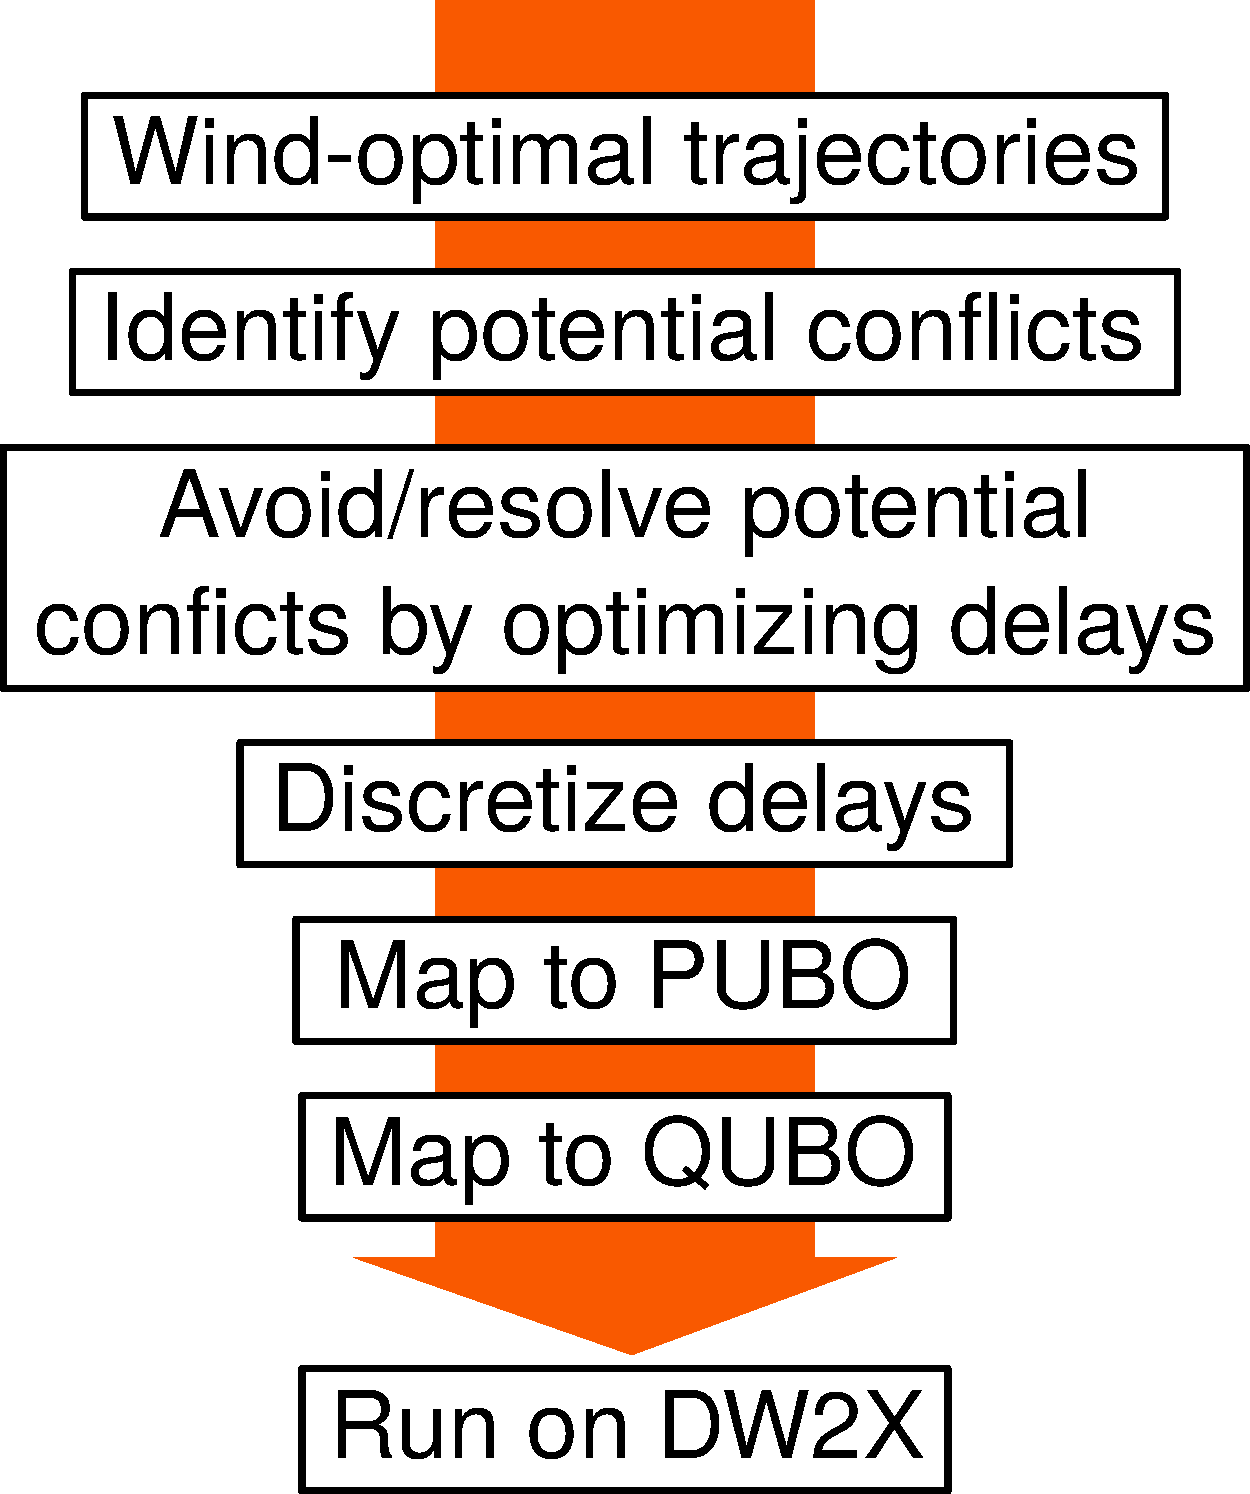
\includegraphics[width=0.25\textwidth]{scheme}
\caption{\label{fig:scheme}Schematic flow diagram to map ATM problems onto the \DW quantum chip. Green/light-gray and orange/dark-gray boxes represent
respectively completed and partially completed tasks.}
\end{wrapfigure}
%
NAT dataset consists in 984 wind-optimal trajectories in (3+1)-dimensions. Since wind-optimal
trajectories have been computed independently from each others, two or more trajectories can intersect in space creating a ``conflict''. 
A conflict becomes ``potential'' if two or more flights can reach at the \emph{same} time the spatial conflict. The ATM problem consists
in finding minimal changes of the wind-optimal trajectories to avoid all the potential conflicts. 
Given the fixed architecture and the limited amount of physical resources of the current quantum hardware, it is impossible to directly solve ATMs problems
on quantum annealers. For this reason, we have designed a series of transformation of the original ATM formulation 
to be able to optimize ATM problems on state-of-art quantum optimizers like the \DW quantum chip. \figurename~\ref{fig:scheme} summarizes the transformation 
we developed in this project (green/light-green and orange/dark-green represent respectively the completed and partially completed tasks).
Here follows a detailed description of the work that has been completed in the period April-June 2016 (3.5 months):

\begin{changemargin}{0.5cm}{0cm}
\textbullet~\textbf{Identify potential conflict.} In principle, any conflict is a potential conflict: indeed, flights can accumulate delay
and therefore arrive at the same to a spatial conflict. Nevertheless, the number of spatial conflicts is prohibitive. To limit the number
of potential conflicts, we pre-processed the wind-optimal trajectories in the following way:
\begin{enumerate}
    \item Pool together potential conflicts which are subsequent in time and space.
    \item Assume that the flights can not have a delay which exceeds 1 hour and then eliminate all the potential conflicts that do not respect the bound.
    \item Reduce the number of of potential conflict even further by the following self-consistent algorithm:
    \begin{enumerate}
        \item \label{itm:algo_order}For each flight, order the potential conflicts in time.
        \item \label{itm:algo_maxDelay} For each flight, calculate the maximal delay which can be picked up due to anteceding conflict avoiding maneuvers.
        \item \label{itm:algo_potConf}For each potential conflict, check if a real conflict is possible considering the maximal delays of the involved flights calculated in step \ref{itm:algo_maxDelay}.
        \item \label{itm:algo_removePotConf}Remove the potential conflicts which can not become real.
        \item Repeat the above steps \ref{itm:algo_order} to \ref{itm:algo_removePotConf} until convergence (i.e.\ the number of potential conflicts is invariant).
    \end{enumerate}
\end{enumerate}
This process drastically reduced the number of potential conflicts from
33878 to 4168.
The code to pre-process the wind-optimal trajectories has
been developed by Tobias Stollenwerk.
\end{changemargin}

\begin{changemargin}{0.5cm}{0cm}
\textbullet~\textbf{Avoid/resolve potential conflicts by optimizing delays/Discretize delays.} Even after the reduction of potential conflicts, it would be impossible to directly
map the (3+1)-dimensional trajectories onto the \DW quantum chip. Instead, we formulate the ATMs in terms of a ``delay'' problem. More precisely,
let us define the time $T_{ik}$ of a flight $i$ to reach a potential conflict $k$, that is:
\begin{equation}\label{eq:T}
	T_{ik}(d_i,\,\left\{d_{ip}\right\}) = t_{ik} + d_i + \sum_{p\in \mathcal{P}^{<k}_i} d_{ip},
\end{equation}
with $t_{ik}$ the wind-optimal time to reach the conflict $k$, $d_i$ the delay at the departure, 
$\mathcal{P}^{<k}_{i}$ the set of potential conflicts $p$ that antecede the conflict $k$ and $d_{ip}$ the delay
of flight $i$ at the potential conflict $p$. In the above formulation, it is assumed that all the maneuvers to avoid potential conflicts
consist in small and local changes of the wind-optimal trajectories that do not create a cascade of new potential conflicts and do not
change the location of the existing potential conflicts. Therefore, we can express the cost function to optimize as
\begin{equation}\label{eq:f}
	f(\left\{d_i\right\},\,\left\{d_{ip}\right\})= \sum_{i} d_i + \sum_{ip} d_{ip},
\end{equation}
where all the $\left\{d_i\right\}$ and $\left\{d_{ip}\right\}$ are constrained so that two flights $i$ ($j$) must have a different arrival time
$T_{ik}$ ($T_{jk}$) to the same potential conflict $k$, namely
\begin{equation}\label{eq:theta}
	\Theta_{a_{ijk}}(\left|T_{ik} - T_{jk}\right|) = 0,
\end{equation}
with $\Theta$ a certain function which ensure that the two flights are sufficiently far apart to complete their maneuvers. Here, $a_{ijk}$ represent
some extra-parameters that can be added to the model to have more control on the maneuvers.\\

\hspace{0.4cm}The delay model is completely defined by the \equationname{s}~(\ref{eq:T})-(\ref{eq:theta}). The successive step
consists in the discretization of the variables involved in the delay model. The discretization is achieved by expressing each variable $x$ in terms 
of a discrete set of values $\left\{x_\alpha\right\}$
\begin{equation}\label{eq:discr}
	x = \sum_{\alpha} x_{\alpha}\sigma_\alpha,
\end{equation}
with $\sigma_{\alpha} = \{0,\,1\}$, and then enforcing that only one among all the $\left\{\sigma_\alpha\right\}$ is one, namely
\begin{equation}\label{eq:constr}
	\sum_\alpha \sigma_\alpha = 1.
\end{equation}
The delay model formulation has been devised by Bryan O'Gorman,
in collaboration with Tobias Stollenwerk, Salvatore Mandr\`a, Davide Venturelli and Eleanor G. Rieffel.
\end{changemargin}

\begin{changemargin}{0.5cm}{0cm}
\textbullet~\textbf{Map to PUBO/QUBO.} The delay model, as expressed in \equationname~(\ref{eq:f}), is a polynomial unconstrained binary optimization (PUBO)
because some of the terms involved are polynomials of order higher than $2$.
However, most of the quantum annealers, including the \DW quantum chip, can only natively solve quadratic unconstrained binary optimization (QUBO) problems,
where only quadratic terms are present.
In order to reduce the PUBO formulation of the delay model to a QUBO formulation, we are devising two different approaches.
The first approach is to use gadgets to reduce higher order polynomials to quadratic terms \cite{babbush:13}. The second approach consists in using Lagrange multipliers \cite{ronagh:15} to enforce constraints as in \equationname~(\ref{eq:constr}) and then reduce the number of higher order polynomials. The two approaches can be
either used independently or mixed together. Salvatore Mandr\`a, Davide Venturelli, Bryan O'Gorman and Eleanor G. Rieffel 
are working in finding a suitable reduction for ATM problems.
\end{changemargin}

\begin{changemargin}{0.5cm}{0cm}
\textbullet~\textbf{Define benchmark.} Given the limited amount of resources of the current quantum technology, it is necessary to identify benchmark problems to
explore the potentiality of quantum annealing. Instances in 
the benchmark ensemble must be small enough to be optimized by the current quantum hardware, like the \DW quantum chip,
but they must be still representative of the hardness of typical size ATM problems. We are devising benchmark instances by using two different approaches. On one
hand, we are looking at ATM-like instances with a reduced number of potential conflicts (e.g. considering only a subset of the total wind-optimal trajectories),
so that the instances can be optimized by the current architecture of quantum chips. On the other hand, we are looking at archetypal spin glass problems \cite{venturelli:15a}
which are not ATM problems but share with them common structures and hardness. The benchmark analysis 
is conducted by Salvatore Mandr\`a, Davide Venturelli and Eleanor G. Rieffel.
\end{changemargin}

\section*{Outlook and next steps}\label{sec:ass}

In the first part of the project, we mainly focused on the formulation of ATM problems in terms of binary optimization problems. More precisely,
We have devised the delay model to reduce ATM problems to a quadratic binary optimization problem (QUBO), which are natively solved by typical 
quantum annealers like the \DW quantum chip. Despite its simplicity, the model can still capture many of the properties of ATM problems. \\

Next step of the project will be to devise a benchmark set of ATM instances and analyze the quality/variety of the solutions of the delay model using 
state-of-art classical QUBO optimizers. This will give us a bottom line for the performance of quantum annealers. Successively, we 
we will run the ATM benchmark set on the current \DW quantum chip and compare the quality of results with the classical counterpart. Given the limited
amount of resources for the \DW quantum chip, the potential quantum enhancement for large system size will
be extrapolate from the data. The results of the \DW quantum chip will be used to identify advantages and bottlenecks of
the current quantum architecture. Finally, driven by the results from both classical and quantum optimizers, 
we will explore different quantum architectures and hardware changes to achieve better performances for quantum optimizers.\\

For a complete overview of completed tasks and future milestones, see \tablename~\ref{table:milestone}.

\section*{Project outputs}

\begin{itemize}
	\item Code to analyze the wind-optimal trajectories and identify potential conflicts within given a maximum delay time.
	\item Mapping of the ATM problem to PUBO.
	\item Reduction from PUBO to QUBO.
\end{itemize}

\begin{table}[h!]\centering
	\begin{tabular}{|m{7cm}|m{7cm}|K{2.8cm}|}
		\rowcolor{gray!30}
		\hline
		\multicolumn{1}{|c|}{\textbf{Task/Milestone}} & \multicolumn{1}{c|}{\textbf{Performance Metric}} & \textbf{Expected completion from start of project}\\
		\hline
		\rowcolor{green!30}
			Devise a code to analyze spatial conflicts and identify potential conflicts within a certain amount of delay. &
				Largest set of trajectories that the code can analyze. Overall performance of the code. & 1.5 month \\
		\hline
		\rowcolor{green!30}
			Analyze the wind-optimal NAT trajectories to identify potential conflicts.
			& Number of potential conflicts. & 2 month \\
		\hline
		\rowcolor{green!30}
			Map the ATM problem to a suitable polynomial binary optimization problem (PUBO). & 
				Number of required qubits. Largest degree of the polynomials. Connectivity of the underlying coupling graph. & 3 month\\
		\hline
		\rowcolor{orange!50}
			Identify suitable approaches to reduce the degree of the polynomials in the PUBO formulation & 
				Overhead of the reduction. & 4 month \\
		\hline
		\rowcolor{orange!50}
			Map the ATM problem to a suitable quadratic binary optimization problem (QUBO). &
				Number of required qubits. Connectivity of the underlying coupling graph. & 5 month\\
		\hline
		\rowcolor{orange!50}
			Identify a set of benchmark ATM problems. & Hardness as a function of size. & 6.5 month\\
		\hline
			Analyze the results/performance of classical QUBO solvers on ATM problems. & 
				Assess the quality/variety of the solutions after discretization. Find the bottom line for classical computation. & 8 month\\
		\hline
			Compile the ATM benchmark ensemble for the \DW chip. & 
				Scaling of expected time to solution vs. size compared to classical code. Variety of different acceptable solutions. &10 month\\
		\hline
			Compare results/quality of solutions of the \DW chip against classical solvers & Potential quantum enhancement & 11 month\\
		\hline
			Outlook on different architectures and annealing strategies, hardware changes &
				Potential quantum enhancement. & 12 month\\
		\hline
	\end{tabular}\caption{\label{table:milestone}Breakdown of the project effort into milestones, including suggested performance metric and completion
		dates (green/light-grey and orange/dark-grey represent respectively completed and partially completed tasks).}
\end{table}

\bibliographystyle{unsrt}
\bibliography{refs.bib}

\end{document}
